\documentclass{article}
\usepackage{graphicx} %for inserting image
\setlength{\parindent}{20pt}
\usepackage[a4paper, margin=3cm]{geometry}
\usepackage[utf8]{inputenc}
\usepackage[T1]{fontenc}
\usepackage[french]{babel}
\usepackage{geometry}  


\begin{document}
\begin{titlepage}
    \centering
    \vspace*{\fill}

    {\Huge \textbf{Software Requirements Document:}\\[0.5cm]
    \textbf{Tetris Royal}} \\[1.5cm]
    
    {\Large Tao Chau\\
    Juliete Cornu-Besser\\
    Quentin Bernard Bouissières\\
    Jonas Schellekens\\
    Ethan Van Ruyskenvelde\\
    Lucas Verbeiren\\
    Ernerst Malysz\\
    Rafaou Gajewicz} \\[2cm]

    {\Large 13 décembre 2024}

    \vspace*{\fill} 
\end{titlepage}

\newpage

\tableofcontents

\newpage

\section{Introduction}

\subsection{But du projet}

\quad Ce projet a pour objectif de concevoir une application de jeu intégrant diverses fonctionnalités multijoueur. Les règles des parties reprendront celles existantes dans \textit{Tetris Royal}, une extension de la version normale du jeu \textit{Tetris}. Chaque joueur possède une grille vide qu'il doit essayer de remplir en laissant le moins d'espace possible avec des \textit{tetriminos}, des formes géométriques qui peuvent être tournés et déplacés avant leur place finale. Les pièces tombent depuis le haut de la grille et plus la partie avance, plus elles tombent rapidement. Une ligne remplie de  \textit{tetriminos} se supprime et fait gagner des points au joueur. La partie se termine quand le joueur ne sait plus placer de formes géométriques sur la grille car il y a des \textit{tetriminos} sur toute la hauteur de la grille. Son score dépendra du temps de la partie et des lignes supprimées.  

\paragraph*{}

Dans cette application, quatre modes sont proposés au joueur. Il existe la version \textit{Endless} avec un seul joueur où le but est de savoir placer des pièces sur la grille le plus longtemps possible. Selon les combinaisons des pièces qui se suppriment, les points attribués seront différents.
 
\paragraph*{}

Puis nous implémentons les modes multijoueurs. Une nouvelle notion doit être introduite : "\textit{une ligne de malus}". Un joueur peut envoyer un malus à un adversaire. Le receveur du malus retrouvera toutes ses lignes poussées vers le haut pour laisser la place à une ou plusieurs rangées avec un bloc manquant en dessous, qui ne peuvent pas être supprimés par les combinaisons.  

\paragraph*{}

La version \textit{Classic} et la version \textit{Duel} comprennent respectivement des parties de trois à neuf, et de deux joueurs. Chaque participant a sa propre grille avec ses \textit{tetriminos} qui tombent; celui qui complète une ou plusieurs lignes en même temps peut envoyer des lignes de malus selon sa combinaison à un adversaire de son choix. 

\paragraph*{}

Le dernier mode, \textit{ Royal Competition}, comprend des malus multiples et des bonus. Ce sont des parties de trois à neuf joueurs. Chaque individu aura sa propre barre d'énergie initialement nulle. Au fil de la partie, la barre se remplie selon les combinaisons de lignes supprimées du joueur. Une fois cette dernière complétée, le joueur peut envoyer des malus à un adversaire ou s'octroyer un bonus qui lui facilite, qui le protège durant un moment. Dans la liste étendue de malus et de bonus, nous retrouvons un ralentissement de la chute des \textit{tetriminos} pour soi-même, augmenter cette vitesse pour un adversaire ou encore inverser les commandes d'action d'un adversaire.

\paragraph*{}

En dehors des parties de jeux, le joueur peut se connecter ou créer un compte pour accéder au \textit{Tetris Royal}. Cela lui permet de gérer sa liste d'amis et de discuter avec eux via une messagerie intégrée à l'application. Il peut également consulter le classement des autres joueurs dans le mode \textit{Endless}. Pour terminer, il peut créer ou rejoindre une partie dans un mode multijoueur sélectionné. Les participants peuvent être invités en mode observateur ou en mode joueur.

\newpage

\subsection{Glossaire}


\begin{itemize}
	\item \textbf{Bonus} : Avantage obtenu par le joueur lorsque celui-ci dépense son énergie. Un bonus peut prendre plusieurs formes comme réduire un tetramino en bloc de 1 x 1 , ou réduire son temps de chute. 
	\item \textbf{Malus} : Pénalité infligée à un joueur par un de ses adversaires. Le malus se manifeste par l'ajout d'une ou de plusieurs lignes supplémentaires en bas de la grille du receveur, poussant les blocs existants vers le haut et rapprochant le joueur de la défaite.
	\item \textbf{Tetriminos} : Pièce de jeu composée de quatre blocs carré connectés entre eux de manière à former différentes formes géométriques, respectivement (Z, L, O, S, I, J, T). 
        \item \textbf{Matchmaking} : Système qui permet de connecter plusieurs joueurs ensemble pour pouvoir créer et lancer une partie en ligne.
        \item \textbf{Pseudo} : Nom utilisé par un utilisateur et qui peut ne pas être son nom officiel.
	
\end{itemize}

\subsection{Historique}

\newpage

\section{Besoins utilisateurs : Fonctionnels}

\subsection{Écran de connexion}

\begin{figure}[!h]
    \centering
    	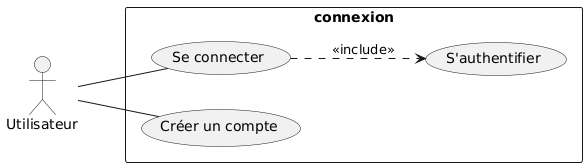
\includegraphics[width=0.9\textwidth]{uml/usescase/connexion/connexion.png}
    	\caption{Diagramme Use Case du Menude Connexion}
    	\label{fig:main-menu}
\end{figure}
Le premier écran que l'utilisateur accède est un moyen de se connecter à la plateforme de jeu via un compte. Le moyen de s'authentifier est avec un compte existant et le mot de passe associé valide. Si l'utilisateur ne possède pas de compte existant, il peut se créer un nouveau compte avec un pseudo non existant sur la plateforme.


\subsubsection*{Connexion}
\begin{itemize}
    \item \textbf{Acteur}: Utilisateur
    \item \textbf{Use case}: Se connecter
    \item \textbf{Description}: Permet à l'utilisateur de se connecter au système.
    \item \textbf{Précondition}: L'utilisateur possède déjà un compte.
    \item \textbf{Postcondition}: L'utilisateur est connecté au système.
    \item \textbf{Cas exceptionnels}: Mauvais identifiant ou mot de passe, échec de la connexion réseau.
\end{itemize}

\subsubsection*{Créer un compte}
\begin{itemize}
    \item \textbf{Acteur}: Utilisateur
    \item \textbf{Use case}: Créer un compte
    \item \textbf{Description}: Permet à un utilisateur de s’inscrire et de créer un compte.
    \item \textbf{Précondition}: L’utilisateur n’a pas encore de compte.
    \item \textbf{Postcondition}: Un nouveau compte est créé et l'utilisateur est authentifié.
    \item \textbf{Cas exceptionnels}: L'utilisateur existe déjà, erreurs de validation de données.
\end{itemize}

\subsubsection*{S'authentifier}
\begin{itemize}
    \item \textbf{Acteur}: Utilisateur
    \item \textbf{Use case}: S'authentifier
    \item \textbf{Description}: Vérifie les informations d'identification fournies par l'utilisateur.
    \item \textbf{Précondition}: L'utilisateur a soumis ses identifiants.
    \item \textbf{Postcondition}: Authentification réussie, session utilisateur créée.
    \item \textbf{Cas exceptionnels}: Identifiants incorrects, serveur d’authentification indisponible.
\end{itemize}

\newpage

\subsection{Menu Principal}

\begin{figure}[!h]
    \centering
    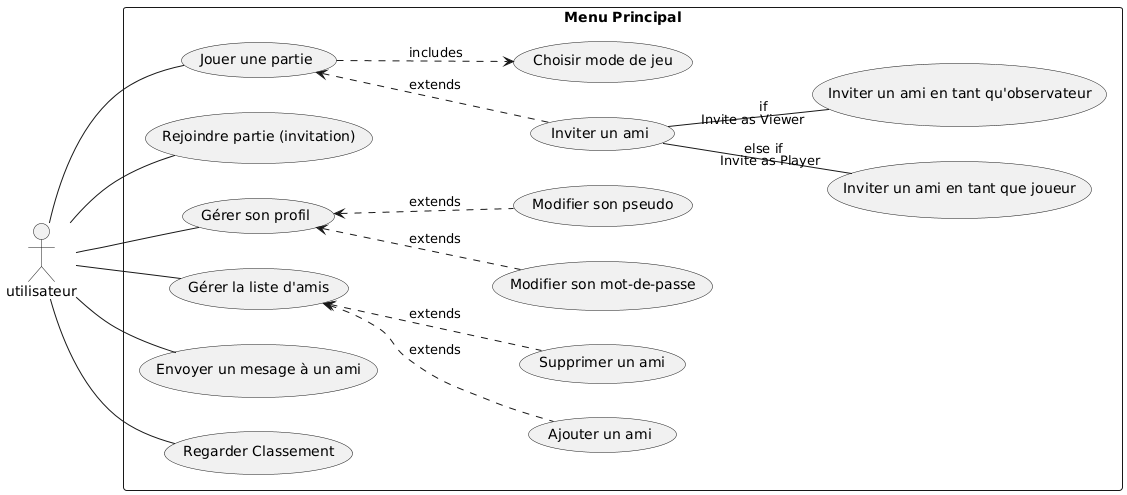
\includegraphics[width=1\textwidth]{uml/usescase/menu-principal/menu_principal.png}
    \caption{Diagramme Use Case du Menu Principal}
    \label{fig:main-menu}
\end{figure}

Une fois l'authentification validée, l'écran du menu principal est accessible. L'utilisateur peut lancer à une partie, gérer son profil, communiquer avec ses amis par la messagerie interne, gérer sa liste d'amis et regarder le classement général du jeu.

\subsubsection*{Jouer une partie}
\begin{itemize}
    \item \textbf{Acteur}: Utilisateur
    \item \textbf{Use case}: Jouer une partie
    \item \textbf{Description}: Permet à l'utilisateur de lancer une partie.
    \item \textbf{Précondition}: L'utilisateur est authentifié.
    \item \textbf{Postcondition}: Une partie de jeu est démarrée.
    \item \textbf{Cas exceptionnels}: Problème de connexion ou erreurs de lancement.
\end{itemize}

\subsubsection*{Rejoindre une partie existante}
\begin{itemize}
    \item \textbf{Acteur}: Utilisateur
    \item \textbf{Use case}: Rejoindre partie existante
    \item \textbf{Description}: Permet à l'utilisateur de rejoindre une partie existante sur invitation d'un ami.
    \item \textbf{Précondition}: L'utilisateur a reçu une invitation.
    \item \textbf{Postcondition}: L'utilisateur rejoint la partie.
    \item \textbf{Cas exceptionnels}: Invitation expirée ou la partie a atteint le nombre maximum de personnes.
\end{itemize}

\subsubsection*{Inviter un ami}
\begin{itemize}
    \item \textbf{Acteur}: Utilisateur
    \item \textbf{Use case}: Inviter un ami
    \item \textbf{Description}: Permet à l'utilisateur d'inviter un de ses amis présents dans sa liste à une partie.
    \item \textbf{Précondition}: L'ami est connecté.
    \item \textbf{Postcondition}: L'invitation est envoyée à l'ami.
    \item \textbf{Cas exceptionnels}: L'ami est indisponible ou n'accepte pas l'invitation.
\end{itemize}

\subsubsection*{Choisir mode de jeu}
\begin{itemize}
    \item \textbf{Acteur}: Utilisateur
    \item \textbf{Use case}: Choisir mode de jeu
    \item \textbf{Description}: Permet à l'utilisateur de choisir le mode de jeu.
    \item \textbf{Précondition}: L'utilisateur veut créer une partie de jeu.
    \item \textbf{Postcondition}: Le mode de jeu est défini pour la partie.
    \item \textbf{Cas exceptionnels}: Aucun.
\end{itemize}

\subsubsection*{Gérer son profil}
\begin{itemize}
    \item \textbf{Acteur}: Utilisateur
    \item \textbf{Use case}: Gérer son profil
    \item \textbf{Description}: Permet à l'utilisateur de modifier les informations de son profil.
    \item \textbf{Précondition}: L'utilisateur est authentifié.
    \item \textbf{Postcondition}: Les informations de profil sont mises à jour.
    \item \textbf{Cas exceptionnels}: Échec de la mise à jour des informations.
\end{itemize}

\subsubsection*{Gérer la liste d'amis}
\begin{itemize}
    \item \textbf{Acteur}: Utilisateur
    \item \textbf{Use case}: Gérer la liste d'amis
    \item \textbf{Description}: Permet à l'utilisateur de gérer sa liste d'amis.
    \item \textbf{Précondition}: L'utilisateur est connecté.
    \item \textbf{Postcondition}: La liste d'amis est mise à jour.
    \item \textbf{Cas exceptionnels}: Problèmes de synchronisation, ami introuvable.
\end{itemize}

\subsubsection*{Envoyer un message à un ami}
\begin{itemize}
    \item \textbf{Acteur}: Utilisateur
    \item \textbf{Use case}: Envoyer un message à un ami
    \item \textbf{Description}: Permet à l'utilisateur d'envoyer un message à un ami.
    \item \textbf{Précondition}: L'ami est dans la liste d'amis.
    \item \textbf{Postcondition}: Le message est envoyé avec succès.
    \item \textbf{Cas exceptionnels}: Ami déconnecté ou problème de réseau.
\end{itemize}

\subsubsection*{Modifier son mot-de-passe}
\begin{itemize}
    \item \textbf{Acteur}: Utilisateur
    \item \textbf{Use case}: Modifier son mot-de-passe
    \item \textbf{Description}: Permet à l'utilisateur de changer son mot de passe.
    \item \textbf{Précondition}: L'utilisateur est authentifié.
    \item \textbf{Postcondition}: Le mot de passe est modifié avec succès.
    \item \textbf{Cas exceptionnels}: Mot de passe actuel incorrect, validation échouée.
\end{itemize}

\subsubsection*{Modifier son pseudo}
\begin{itemize}
    \item \textbf{Acteur}: Utilisateur
    \item \textbf{Use case}: Modifier son pseudo
    \item \textbf{Description}: Permet à l'utilisateur de changer son pseudo.
    \item \textbf{Précondition}: L'utilisateur est authentifié.
    \item \textbf{Postcondition}: Le pseudo est modifié avec succès.
    \item \textbf{Cas exceptionnels}: Le pseudo est déjà pris, le changement de pseudo est invalidé.
\end{itemize}

\subsubsection*{Ajouter un ami}
\begin{itemize}
    \item \textbf{Acteur}: Utilisateur
    \item \textbf{Use case}: Ajouter un ami
    \item \textbf{Description}: Permet à l'utilisateur d'ajouter un autre utilisateur à sa liste d'amis.
    \item \textbf{Précondition}: Le potentiel nouveau ami existe et est accessible.
    \item \textbf{Postcondition}: L'utilisateur est ajouté en tant qu'ami dans sa nouvelle liste.
    \item \textbf{Cas exceptionnels}: Ami déjà présent dans la liste ou utilisateur introuvable.
\end{itemize}

\subsubsection*{Supprimer un ami}
\begin{itemize}
    \item \textbf{Acteur}: Utilisateur
    \item \textbf{Use case}: Supprimer un ami
    \item \textbf{Description}: Permet à l'utilisateur de retirer un ami de sa liste.
    \item \textbf{Précondition}: L'ami existe dans la liste d'amis.
    \item \textbf{Postcondition}: L'ami est supprimé de la liste.
    \item \textbf{Cas exceptionnels}: L'utilisateur à supprimer n'est pas dans la liste d'amis.
\end{itemize}

\subsubsection*{Inviter un ami en tant que joueur}
\begin{itemize}
    \item \textbf{Acteur}: Utilisateur
    \item \textbf{Use case}: Inviter un ami en tant que joueur
    \item \textbf{Description}: L'utilisateur a créé une partie et invite un joueur dans sa liste d'amis dans la partie.
    \item \textbf{Précondition}: L'ami est connecté.
    \item \textbf{Postcondition}: Invitation envoyée pour jouer.
    \item \textbf{Cas exceptionnels}: L'ami n'est pas disponible et l'invitation est rejetée.
\end{itemize}

\subsubsection*{Inviter un ami en tant qu'observateur}
\begin{itemize}
    \item \textbf{Acteur}: Utilisateur
    \item \textbf{Use case}: Inviter un ami en tant qu'observateur
    \item \textbf{Description}: L'utilisateur a créé une partie et invite un ami de sa liste d'amis à la partie en tant qu'observateur.
    \item \textbf{Précondition}: L'ami est connecté.
    \item \textbf{Postcondition}: Invitation envoyée pour observer.
    \item \textbf{Cas exceptionnels}: L'ami est indisponible et l'invitation est rejetée.
\end{itemize}

\subsubsection*{Regarder Classement}
\begin{itemize}
    \item \textbf{Acteur}: Utilisateur
    \item \textbf{Use case}: Regarder Classement
    \item \textbf{Description}: Permet à l'utilisateur de consulter les classements.
    \item \textbf{Précondition}: L'utilisateur est connecté.
    \item \textbf{Postcondition}: Le classement est affiché.
    \item \textbf{Cas exceptionnels}: Classement indisponible, problèmes de connexion.
\end{itemize}

\newpage

\subsection{Différents modes de jeux}

\subsubsection{En mode Endless}

\begin{figure}[!h]
    \centering
    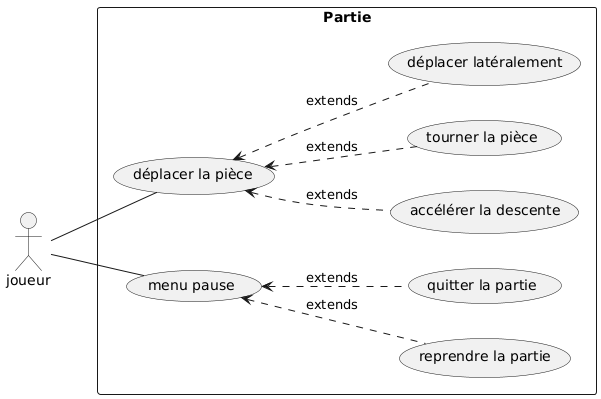
\includegraphics[width=1\textwidth]{uml/usescase/en-jeu/endless.png}
    \caption{Diagramme Use Case en mode Classique}
    \label{fig:Classique}
\end{figure}

\subsubsection*{Déplacer la pièce}
\begin{itemize}
    \item \textbf{Acteur}: Joueur
    \item \textbf{Use case}: Déplacer la pièce
    \item \textbf{Description}: Permet au joueur de déplacer une pièce sur le plateau.
    \item \textbf{Précondition}: Une partie est en cours et le joueur contrôle une pièce.
    \item \textbf{Postcondition}: La pièce est déplacée dans une direction choisie.
    \item \textbf{Cas exceptionnels}: Limite du plateau atteinte, collision avec d'autres pièces.
\end{itemize}

\subsubsection*{Tourner la pièce}
\begin{itemize}
    \item \textbf{Acteur}: Joueur
    \item \textbf{Use case}: Tourner la pièce
    \item \textbf{Description}: Permet au joueur de tourner la pièce dans une direction donnée.
    \item \textbf{Précondition}: Une partie est en cours et une pièce est active.
    \item \textbf{Postcondition}: La pièce est tournée en conséquence.
    \item \textbf{Cas exceptionnels}: La rotation amène la pièce en dehors des limites.
\end{itemize}

\subsubsection*{Menu pause}
\begin{itemize}
    \item \textbf{Acteur}: Joueur
    \item \textbf{Use case}: Menu pause
    \item \textbf{Description}: Permet au joueur d'ouvrir le menu de pause.
    \item \textbf{Précondition}: La partie est en cours.
    \item \textbf{Postcondition}: La partie est en pause.
    \item \textbf{Cas exceptionnels}: Aucun.
\end{itemize}

\subsubsection*{Reprendre la partie}
\begin{itemize}
    \item \textbf{Acteur}: Joueur
    \item \textbf{Use case}: Reprendre la partie
    \item \textbf{Description}: Permet de reprendre la partie après une pause.
    \item \textbf{Précondition}: La partie est en pause.
    \item \textbf{Postcondition}: La partie reprend là où elle s'était arrêtée.
    \item \textbf{Cas exceptionnels}: Aucun.
\end{itemize}

\subsubsection*{Quitter la partie}
\begin{itemize}
    \item \textbf{Acteur}: Joueur
    \item \textbf{Use case}: Quitter la partie
    \item \textbf{Description}: Permet au joueur de quitter la partie en cours.
    \item \textbf{Précondition}: La partie est en cours.
    \item \textbf{Postcondition}: Le joueur quitte la partie et retourne au menu principal.
    \item \textbf{Cas exceptionnels}: Aucun.
\end{itemize}

\subsubsection{En mode Duel}

\begin{figure}[!h]
    \centering
    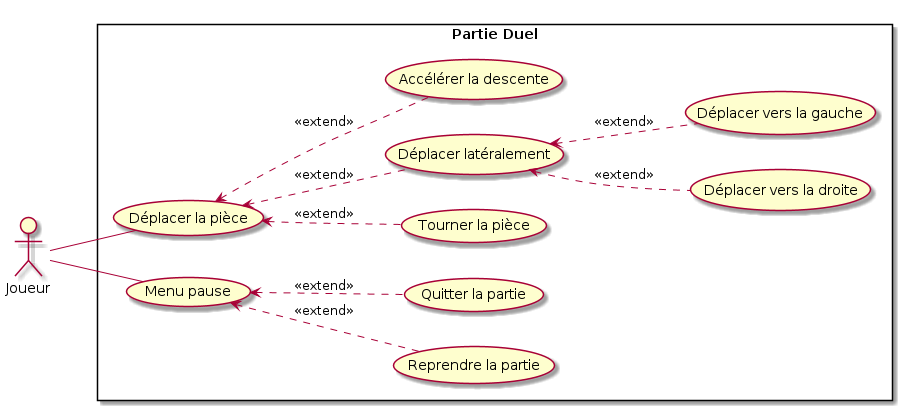
\includegraphics[width=1\textwidth]{uml/usescase/en-jeu/dual.png}
    \caption{Diagramme Use Case en mode Duel}
    \label{fig:Duel}
\end{figure}

\subsubsection*{Déplacer la pièce} (identique au mode Endless)

\subsubsection*{Tourner la pièce} (identique au mode Endless)

\subsubsection*{Envoyer n-1 malus}
\begin{itemize}
    \item \textbf{Acteur}: Joueur
    \item \textbf{Use case}: Envoyer n-1 malus
    \item \textbf{Description}: Envoie une ligne de malus à l'adversaire.
    \item \textbf{Précondition}: Le joueur a complété un nombre spécifique de lignes.
    \item \textbf{Postcondition}: L'adversaire reçoit le malus.
    \item \textbf{Cas exceptionnels}: Échec de l’envoi du malus, conditions de malus non remplies.
\end{itemize}

\subsubsection*{Menu pause}
\begin{itemize}
    \item \textbf{Acteur}: Joueur
    \item \textbf{Use case}: Menu pause
    \item \textbf{Description}: Permet au joueur d'ouvrir le menu de pause.
    \item \textbf{Précondition}: La partie est en cours.
    \item \textbf{Postcondition}: La partie est en pause.
    \item \textbf{Cas exceptionnels}: Aucun.
\end{itemize}

\subsubsection*{Reprendre la partie}
\begin{itemize}
    \item \textbf{Acteur}: Joueur
    \item \textbf{Use case}: Reprendre la partie
    \item \textbf{Description}: Permet de reprendre la partie après une pause.
    \item \textbf{Précondition}: La partie est en pause.
    \item \textbf{Postcondition}: La partie reprend là où elle s'était arrêtée.
    \item \textbf{Cas exceptionnels}: Aucun.
\end{itemize}

\subsubsection*{Quitter la partie}
\begin{itemize}
    \item \textbf{Acteur}: Joueur
    \item \textbf{Use case}: Quitter la partie
    \item \textbf{Description}: Permet au joueur de quitter la partie en cours.
    \item \textbf{Précondition}: La partie est en cours.
    \item \textbf{Postcondition}: Le joueur quitte la partie et retourne au menu principal.
    \item \textbf{Cas exceptionnels}: Aucun.
\end{itemize}

\subsubsection{En mode Classique}

\begin{figure}[!h]
    \centering
    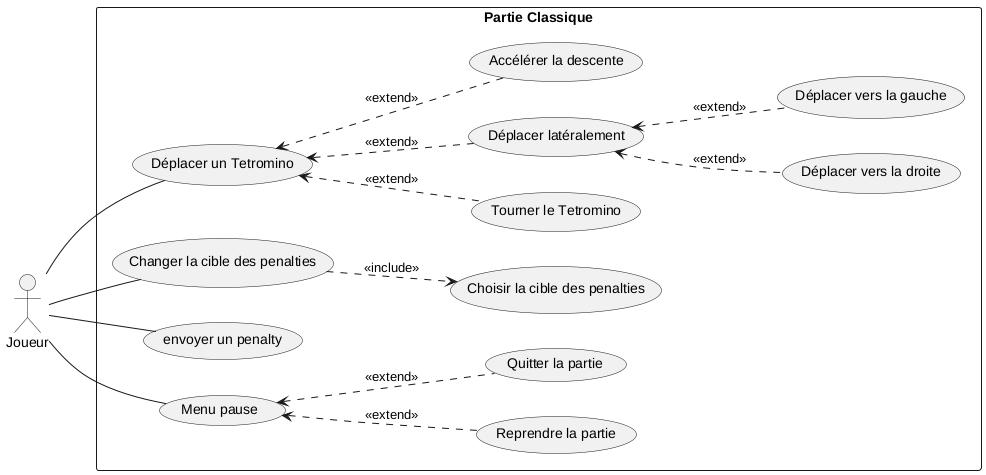
\includegraphics[width=1\textwidth]{uml/usescase/en-jeu/classic.png}
    \caption{Diagramme Use Case en mode Classique}
    \label{fig:Endless}
\end{figure}

\subsubsection*{Déplacer la pièce} (identique à Duel)
\subsubsection*{Tourner la pièce} (identique à Duel)

\subsubsection*{Déplacer latéralement} (identique au mode Endless)

\subsubsection*{Accélérer la descente} (identique au mode Endless)

\subsubsection*{Menu pause} (identique à Duel)
\subsubsection*{Reprendre la partie} (identique à Duel)
\subsubsection*{Quitter la partie} (identique à Duel)

\subsubsection{En mode Royal Competition}

\begin{figure}[!h]
    \centering
    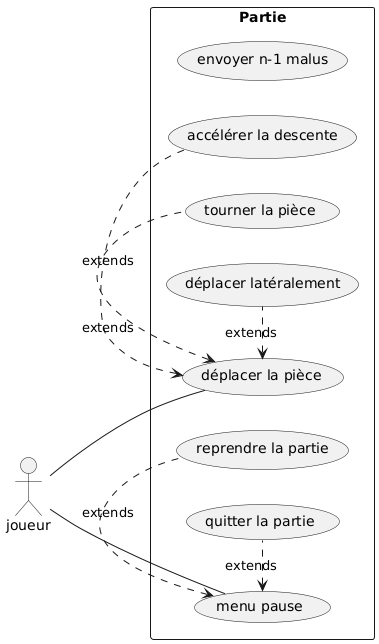
\includegraphics[width=1\textwidth]{uml/usescase/en-jeu/royal-competition.png}
    \caption{Diagramme Use Case en mode Royal Competition}
    \label{fig:Royal-Competition}
\end{figure}

\subsubsection*{Déplacer la pièce} (identique au mode Endless)
\subsubsection*{Tourner la pièce} (identique au mode Endless)
\subsubsection*{Déplacer latéralement} (identique à Endless)
\subsubsection*{Accélérer la descente} (identique à Endless)

\subsubsection*{Envoyer n-1 malus} 
à modifier 

\subsubsection*{Discuter}
\begin{itemize}
    \item \textbf{Acteur}: Joueur
    \item \textbf{Use case}: Discuter
    \item \textbf{Description}: Permet aux joueurs de discuter entre eux pendant la partie.
    \item \textbf{Précondition}: Une partie multijoueur est en cours.
    \item \textbf{Postcondition}: Message envoyé à l'adversaire.
    \item \textbf{Cas exceptionnels}: Connexion interrompue, messages non envoyés.
\end{itemize}

\subsubsection*{Menu pause} (identique à Duel)
\subsubsection*{Reprendre la partie} (identique à Duel)
\subsubsection*{Quitter la partie} (identique à Duel)

\newpage

\section{Besoin système : Fonctionnels}

\subsection{Connexion}

\quad Quand l'utilisateur ouvre l'application, il doit avoir un compte valide pour s'authentifier. Il doit fournir des informations sur le nom du compte et le mot de passe.\\
Ses entrées sur les deux champs sont envoyées au serveur de l'application. Les données sont vérifiées en recherchant sur la base de données un profil correspondant. Si un compte est trouvé avec le mot de passe correctement entré, le serveur connecte l'utilisateur au compte associé. Mais s'il ne trouve pas dans la base de données, l'utilisateur est notifié d'un message d'erreur du serveur.

\subsection{Gestion des comptes}

\subsubsection{Création d'un compte}

Quand un utilisateur crée un compte, il doit fournir un nom de compte et un mot de passe. Chacune de ces entrées saisies a une taille minimale, maximale et une restriction sur les caractères autorisées. Le nom utilisé doit être unique pour chaque compte.\\
Le serveur vérifie qu'il n'existe pas déjà une autre entrée possédant le même nom. 

\subsubsection{Suppression d'un compte}

L'option de suppression du compte doit être possible sur le système. Quand l'utilisateur fait une telle demande en confirmant avec son mot de passe associé, le programme client questionne une dernière fois avant d'envoyer la requête au serveur. Le serveur supprime l'entrée sur la base de données du compte en quetion et l'utilisateur est déconnecté de la session.

\subsection{Consulter le classement}

Quand l'utilisateur est connecté et en dehors d'une partie de jeu, il peut consulter le classement général des joueurs de la plateforme pour le mode de jeu \textit{Endless}. Le serveur l'actualise à chaque fin de partie et l'envoie à chaque requête d'utilisateur concernant le classement.

\subsection{Gestion de la partie}

De la création à la fin de la partie, toutes les actions de l'utilisateur sont envoyées en requête au serveur et ce dernier applique l'action si elle est possible (ex. placer une pièce à tel endroite de la grille, envoyer un malus à un adversaire, etc). Le serveur permet de valider les actions et de vérifier s'il n'y a pas de triche en cours. La partie modifiée par le serveur avec la nouvelle action intégrée ou non sera récupérée et affichée à l'utilisateur.

\subsection{Gestion des amis}

Quand un utilisateur veut rajouter un autre utilisateur existant sur la plateforme à sa liste d'amis, le programme client enverra une requête .

\subsubsection{Gestion du chat}

\subsection{Fin de la partie}

\subsubsection{Fin de la partie normale}

\subsubsection{Fin de la partie Duo}

\subsubsection{Fin de la partie Endless}


\section{Besoins système : Non fonctionnels}

\subsection{Besoins utilisateur}
Le jeu doit proposer une interface graphique facile à utiliser et assez jolie. Le lancement des parties locales et en ligne doit être assez rapide.

\subsection{Besoins système}

\subsubsection{Réseau}
Le jeu doit se jouer en réseau car il a besoin de se connecter au serveur.

\subsubsection{Système d'exploitation}
Le jeu doit pouvoir être lancé sur le système d'exploitation Linux.

\subsubsection{Accessibilité}
Le serveur doit être en ligne pour pouvoir se connecter et accéder au jeu.

\subsubsection{Performances}
Les temps de rafraîchissement et les temps de réponses seront en millisecondes.

\subsubsection{Capacité}
Le jeu pourra lancer une partie jusqu'à neuf joueurs pour le mode classique et acceptera aussi des spectateurs pour voir la partie en cours. L'espace de stockage sera quelques Megabytes.

\subsubsection{Sécurité}
Pour accéder au jeu, l'utilisateur devra s'authentifier à l'aide d'un pseudo et un mot de passe.

\subsubsection{Robustesse}

\newpage

\section{Architecture du système}

\subsection{Architecture du serveur}

\subsection{Architecture du jeu}

\subsection{Architecture du client}

\section{Fonctionnement du système}

\subsection{Création d'un compte}

\subsection{Connexion}

\subsection{Envoi d'une requête}

\subsection{Traitement d'une requête}

\subsection{Lancement d'une partie}

\subsection{Rejoindre un Lobby}


\end{document}